\section{Theoretical Results}

\begin{frame}{Theoretical Work on t-SNE}
    \begin{theorem}[Cluster Formation \cite{LindStein2022}]
        Let $\mathcal{X}$ be "clustered" and initialize $\mathcal{Y} \subset [-0.01, 0.01]^2$. Choose $\alpha$ and $h$ such that for some $1 \leq i \leq n$ \[0.01 \leq \alpha h \sum_{\substack{j \neq i \\ \text{same cluster}}} p_{ij} \leq 0.9\] Then, the diameter of the embedded cluster $\{y_i: 1 \leq j \leq n \land \pi(j) = \pi(i)\}$ decays exponentially until its diameter satisfies, for some universal $c > 0$, 
        \[ \text{diam}\{y_j: 1 \leq j \leq n \land \pi(j) = \pi(i) \} \leq c h \left( \alpha  \sum_{\substack{j \neq i \\ \text{same cluster}}} p_{ij} + \frac{1}{n}\right). \]
    \end{theorem}\pause
    \begin{itemize}
        \item Other theoretical results study connections to spectral clustering (\cite{CaiMa2022}) and limiting behaviour for $n \to \infty$ (\cite{murray2024largedatalimitsscaling}). 
    \end{itemize}
\end{frame}

\begin{frame}{Weaknesses of t-SNE}
    \begin{itemize}
        \item No convergence to global optimum guaranteed due to non-convex loss function \pause
        \item Results heavily depend on choice of parameters \pause 
        \item Visualizations can be misleading  
    \end{itemize}
    \begin{figure}
        \centering
        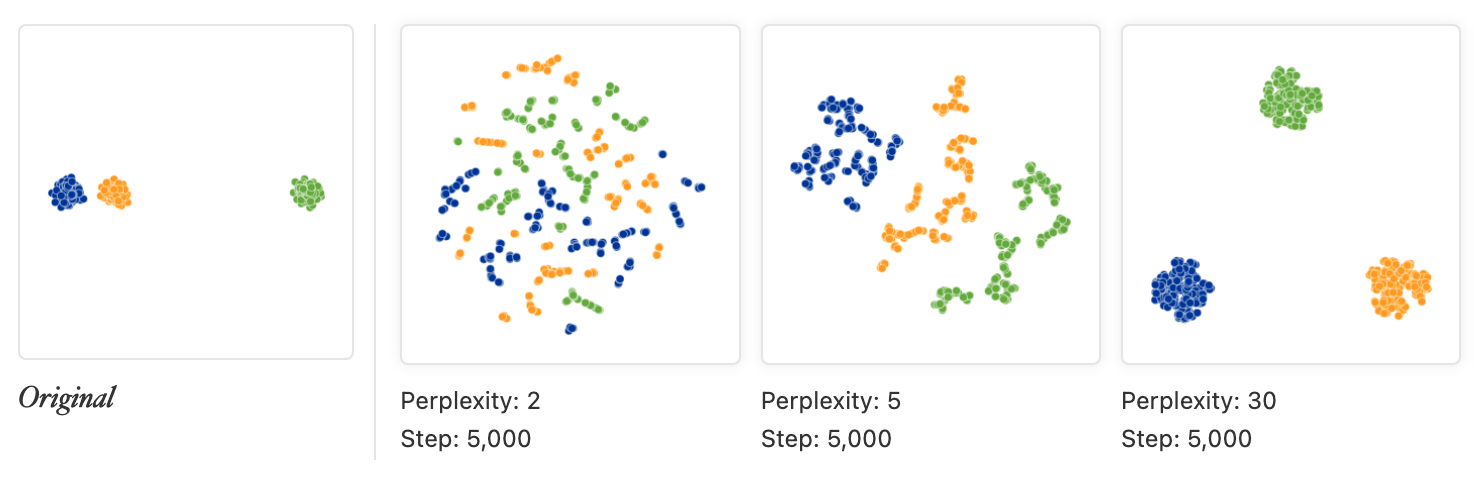
\includegraphics[width=\textwidth]{misread_tsne_1.png}
        \caption{t-SNE does not preserve distance between clusters, see \cite{wattenberg2016how}}. 
    \end{figure}
\end{frame}
 

\begin{frame}{Weaknesses of t-SNE}
    \begin{itemize}
        \item No guaranteed convergence to global optimum due to non-convex loss function 
        \item Results heavily depend on choice of parameters 
        \item Visualizations can be misleading  
    \end{itemize}
    \begin{figure}
        \centering
        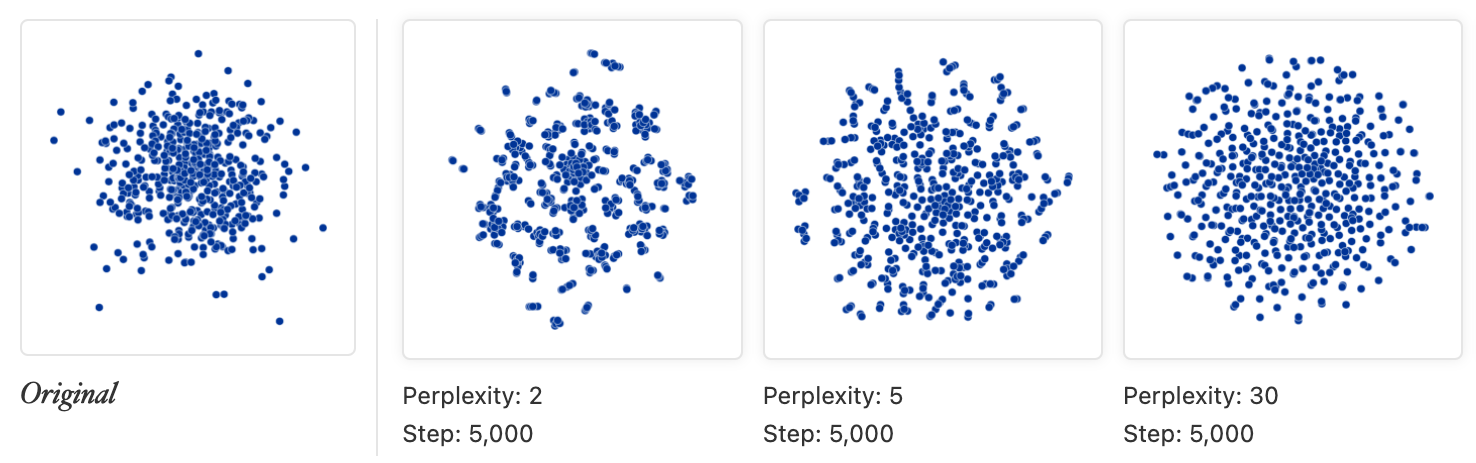
\includegraphics[width=\textwidth]{misread_tsne_2.png}
        \caption{Random Gaussian noise does not always look random, see \cite{wattenberg2016how}}. 
    \end{figure}
\end{frame}

